\chapter{Les cinq piliers de l'islam}
\label{5pilliers}
L'islam repose sur cinq piliers, sur cinq fondements. Il y a~:

\begin{Def}[5 pilliers de l'Islam].

\begin{itemize}
\item
  la \emph{šahāda}, c'est-à-dire l'attestation de foi
\item
  la \emph{ṣalāt}, c'est-à-dire la prière
  La~\emph{salât},~\emph{salâh}~(صلاة {[}ṣalāʰ{]}) ou~\emph{namaz}
\item
  la \emph{zakāt}, c'est-à-dire l'impôt religieux. Éviter de traduire
  \emph{zakāt} par aumône.
\item
  le \emph{ṣiyām}, c'est-à-dire le jeûne
\item
  le \emph{ḥaǧǧ}, c'est-à-dire le pèlerinage
\end{itemize}
\end{Def}

Ces piliers sont eux-mêmes fondés sur le Coran et la Sunna. En effet, la
Sunna de Buḫārī ou celle de Muslim rapportent le propos du prophète
Muḥammad selon lequel, «~l'islam est fondé sur cinq piliers
(\emph{arkān})~». Si la réalité du jeûne, de la prière, etc. se
retrouvent dans le Coran, la détermination de cinq piliers n'est pas
coranique~; elle ne se trouve que dans la Sunna. Ces piliers ont une
valeur religieuse importante dans la mesure où c'est en les
accomplissant que le musulman éprouve l'expérience la plus forte de son
appartenance à l'islam. Le musulman accomplit les piliers, et ainsi il
peut se dire musulman. Mais l'acte d'islam n'est pas que pure pratique
extérieure. Il s'agit d'obéir à Dieu, de le suivre, de se purifier de
ses idoles. Il n'y a pas d'autres dieux que Dieu affirme le musulman
dans la \emph{šahāda.} Tous les autres piliers sont une déclinaison de
cette attestation de foi, de ce témoignage de foi.

Dans ce chapitre, nous allons exposer la valeur spirituelle de ces
piliers et de leur implication pour la vie du croyant en suivant l'un
des maîtres de l'islam~: al-Ġazālī \label{theol:AlGazali10}. La somme spirituelle \emph{Iḥyāʾ
ʿulūm al-dīn}, consacre un livre à chacun de ces piliers.



\vide{i.-la-ux161ahux101da-et-la-double-profession-de-foi}{%
\section{La šahāda et la double profession de
foi}\label{i.-la-ux161ahux101da-et-la-double-profession-de-foi}}

«~Je témoigne qu'il n'y a nul Dieu adoré sinon Dieu et je témoigne que
Muḥammad est le Messager de Dieu~».



\mn{La šahāda en arabe}

\vide{formulation}{%
\subsection{Formulation}\label{formulation}}

La \emph{šahāda} est le premier pilier de l'islam. C'est en la
prononçant que l'on devient musulman. C'est le `baptême musulman', mais
vous voyez que la comparaison est très maladroite : par exemple, dans le
baptême les paroles sont prononcées par le prêtre, dans la
\emph{šahāda}, les paroles sont prononcées par le croyant lui-même,
devant témoins.

Elle est une double attestation~: il s'agit d'attester à la fois
l'unicité divine et de reconnaître la mission prophétique de Muḥammad.

La formule consacrée est «~\emph{ašhadu an lā ilāha illā Llāh}~\emph{wa
ašhadu anna Muhammadan rassūl Allāh} ».

Le mot \emph{šahāda} est constitué de la racine ša.ha.da qui sert dans
la formation des mots \emph{šāhid}, le témoin et \emph{šahīd}, le
martyr. Vous voyez l'importance de bien prononcer en arabe la voyelle
longue~: c'est elle qui va donner le sens au mot.

Le verbe est celui de l'attestation, du témoignage. Il est conjugué à la
première personne du singulier~signifiant l'implication personnelle de
celui qui la prononce, à la différence de la formule plus brève~:
«~\emph{lā ilāha illā Llāh}~». Vous vous souvenez, nous avions vu cette
distinction à propos de la théologie de la louange exposée par al-Rāzī
dans son commentaire de la \emph{Fātiha}, la première sourate du Coran.

\vide{origines-coraniques-de-la-ux161ahux101da}{%
\subsection{{1.2 Origines coraniques de la
\emph{šahāda}}{1.2 Origines coraniques de la šahāda}}\label{origines-coraniques-de-la-ux161ahux101da}}

La \emph{šahāda} n'est pas formalisée comme telle dans le Coran mais on
retrouve dans plusieurs versets du Coran son exposé. Ainsi~:

S.~37, 35~: «~Quand on leur disait~: `Point de divinité à part Dieu',
ils se gonflaient d'orgueil ».

S.~4, 136 : «~Croyez en Dieu et en son Prophète, au Livre qu'Il a révélé
à son Prophète, au Livre qu'Il a révélé auparavant. Quiconque ne croit
pas en Dieu, à ses Anges, à ses Livres, à ses prophètes et au Jour
dernier, se trouve dans un profond égarement.~»

S. 49, 15: «~Les vrais croyants sont seulement ceux qui croient en Dieu
et en Son messager, qui par la suite ne doutent point \ldots~»

S. 7, 158 : «~Dis : `Ô hommes~! Je suis pour vous tous le Messager de
Dieu, à qui appartient la royauté des cieux et de la terre. Pas de
divinité à part lui. Il donne la vie et il donne la mort. Croyez donc en
Dieu, en son messager, le Prophète illettré qui croit en Dieu et en ses
paroles. Et suivez-le afin que vous soyez bien guidés'~».

Un verset concerne le serment d'allégeance de la femme croyante. Il
contient la \emph{šāhada}, mais il témoigne d'une plus grande exigence~:

S. 60, 12~: «~Ô Prophète~! Quand les croyantes viennent te prêter
serment d'allégeance {[}et en jurent{]} qu'elles n'associeront rien à
Dieu, qu'elles ne voleront pas, qu'elles ne se livreront pas à
l'adultère, qu'elles ne tueront pas leurs propres enfants, qu'elles ne
commettront aucune infamie ni avec leurs mains ni avec leurs pieds et
qu'elles ne désobéiront pas en ce qui est convenable, alors reçoit leur
serment d'allégeance, et implore le pardon d'Allah pour elles~».

\vide{remarques-et-commentaires-grammaticaux}{%
\subsection{ Remarques et commentaires grammaticaux
}{}\label{remarques-et-commentaires-grammaticaux}}

Dans cette formule, les grammairiens et lexicographes musulmans ont
souligné trois éléments~:

\begin{itemize}
\item
  \emph{lā ilāha~:} c'est une négation absolue
\item
  \emph{illā Llāh}~: c'est une affirmation absolue.
\item
  Nous traduisons de l'arabe par Dieu deux mots pourtant différents~:
  \emph{ilāh} et \emph{Llāh}. Or, il y a bel et bien une différence de
  sens.

  \begin{itemize}
  \item
    Pour certains philologues, Allāh est un nom propre. Il est le nom de
    l'Essence divine. La \emph{šahāda} peut se traduire ainsi~: s'il y a
    un dieu, c'est Dieu.
  \item
    Cependant, d'autres font remarquer que Allāh vient de la racine
    A.L.H ou W.L.H. dont la signification est~: «~être éperdu d'amour,
    avoir la nostalgie de quelque chose, être haut et briller, être
    voilé, être permanent~». Il s'ensuit une attitude lors de
    l'invocation du nom de Dieu~: attitude emprunte d'humilité, de
    nostalgie et d'amour. La prononciation est emphatique et le ā
    devient quasiment un ô. Dans ce cas, le \emph{ilāh} est une
    illusion. S'il y a une réalité divine, ce ne peut être qu'Allāh.
  \end{itemize}
\end{itemize}

Il y a dans cette formule une affirmation religieuse fondamentale~: il
revient en effet au fidèle de s'écarter de tout ce qui n'est pas Allāh
et cela nécessite un combat, c'est le \emph{ǧihād akbar}, le plus grand
combat. Il s'agit d'un combat contre sa propre personne, son âme qui est
enclin au mal. Il s'agit de reconnaître que Dieu n'a pas d'associé,
qu'il est l'Origine de tout. Maurice Gloton dit de cette formule qu'elle
est «~l'expression la plus parfaite de l'Unicité divine et de la Réalité
essentielle et permanente de l'être~»\sn{~Al-Ġazālī, \emph{Les
  secrets du Pèlerinage en Islam}, avec un commentaire des cinq piliers
  de l'Islam, Paris, Al-Bouraq, p. 60.}.

Ecoutez comment Khaled Roumo parle du mot Allah en arabe. C'était à
l'émission de Ghaleb Bencheikh, Questions d'islam, le 16 octobre 2016.
Vous pouvez
\url{https://www.franceculture.fr/emissions/questions-dislam/amour-et-revelation}{écouter}
l'ensemble de l'émission.

\vide{la-deuxiuxe8me-partie-de-la-formule-est-muux1e25ammad-raux1e63ux16bl-alluxe2h}{%
\subsubsection{{La deuxième partie de la formule est
\emph{Muḥammad Raṣūl
Allâh}}{}}\label{la-deuxiuxe8me-partie-de-la-formule-est-muux1e25ammad-raux1e63ux16bl-alluxe2h}}

Muḥammad vient de la racine Ḥa Mi Da et signifie remercier, célébrer les
perfections d'une chose. Cependant, en tant qu'il s'agit d'un participe
passif de la deuxième forme, il signifie produire la louange. Muḥammad
c'est donc celui en qui la louange est produite. Les grammairiens font
aussi remarquer qu'il s'agit d'un nom de temps et de lieu~: Muḥammad
c'est donc le support de la louange pendant un temps~imparti.

Pour les musulmans, Muḥammad est le nom du Prophète qui est le
réceptacle de la louange. C'est le nom le meilleur qui soit et l'on
comprend pourquoi la tradition encourage à ce que l'on appelle les
garçons par ce nom.

\vide{raux1e63ux16bl-ra-si-la.}{%
\paragraph{Raṣūl~: Ra Si La.}\label{raux1e63ux16bl-ra-si-la.}}

Cette racine a des sens multiples. Elle signifie bien sûr envoyer,
missionner (d'où la fameuse \emph{Risala} d'al-Šafiʿī que nous avons vue
au chapitre précédent et qui signifie \emph{Lettre}, \emph{Épître}, tout
simplement), mais aussi avoir le pas lent, avancer de manière gracieuse
comme le chameau, avoir du lait en abondance, avoir la chevelure longue
et flottante.

De tous ces sens, nous en déduisons que le \emph{Raṣūl} est l'envoyé, le
missionné, le mandaté pour accomplir une mission qu'il accomplit avec
constance apportant l'abondance et le bienfait, dissipant les
oppositions.

\vide{les-enseignements-de-luxe9pigraphie-sur-la-ux161ahux101da}{%
\subsection[1.4 Les enseignements de l'épigraphie sur la \emph{šahāda}
]{\vide{1.4 Les enseignements de l'épigraphie sur la
\emph{šahāda}\sn{\textbf{Frédéric} Imbert, «~L'Islam des pierres~:
  l'expression de la foi dans les graffiti arabes des premiers
  siècles~», \emph{Revue des mondes musulmans et de la Méditerranée}
  {[}En ligne{]}, 129~\textbar~juillet 2011, mis en ligne le 10 mai
  2011, consulté le 18 novembre 2014. URL~:
  http://remmm.revues.org/7067.}
}{1.4 Les enseignements de l'épigraphie sur la šahāda }}\label{les-enseignements-de-luxe9pigraphie-sur-la-ux161ahux101da}}

De quand date l'usage de la \emph{šahāda} comme signe d'appartenance à
l'islam~? Sous quelle forme existait-t-elle~? À cette question
l'épigraphie, c'est-à-dire l'étude des inscriptions dans la pierre,
révèle bien l'existence de l'attestation, mais les plus anciennes
inscriptions ne citent pas le prophète Muḥammad. Ces recherches
confirment ce que nous avions déjà vu à la lumière des sources
musulmanes~: une sacralisation progressive de la figure de Muḥammad et
de ses paroles (\emph{ḥadīṯ}). Nous avons aussi parlé de cette question
dans notre première séance à propos du \emph{Coran des historiens}. Vous
vous souvenez~?

\vide{httpwww.canalacademie.comimgjpgimbert_1_graffiti_spip.jpg}{%
{{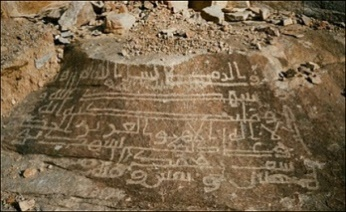
\includegraphics[width=1.57639in,height=0.96528in]{Images/image057.jpg}}{http://www.canalacademie.com/IMG/jpg/Imbert\_1\_graffiti\_SPIP.jpg}}\label{httpwww.canalacademie.comimgjpgimbert_1_graffiti_spip.jpg}}

\vide{graffiti-islamiques-du-duxe9but-de-lislam}{%
\subsubsection{{\textbf{Graffiti islamiques du début de
l'islam}
}{Graffiti islamiques du début de l'islam }}\label{graffiti-islamiques-du-duxe9but-de-lislam}}

\vide{photographie-fruxe9duxe9ric-imbert}{%
\subsubsection{{\textbf{photographie Frédéric
Imbert}}{photographie Frédéric Imbert}}\label{photographie-fruxe9duxe9ric-imbert}}

 

\paragraph{Pour aller plus loin}

Je vous propose de lire l'article de Frédéric Imbert, «~L'Islam des
pierres~: l'expression de la foi dans les graffiti arabes des premiers
siècles~», \emph{Revue des mondes musulmans et de la Méditerranée},
129~\textbar~juillet 2011. Il est consultable en ligne 

Pour vous guider dans sa lecture, une grille de questions~:

§7 et §10. Qu'est-ce que la \emph{basmala}~? Pourquoi l'auteur semble
lui accorder une certaine importance~?

§14. Pourquoi est-il intéressant de noter que la mention du Prophète est
absente~?

§19. Quelle est la thèse et l'argumentation de Y. Nevo à propos de
«~l'évidence de l'absence~»~?

De quand date la première mention du Prophète de l'islam dans un
graffito~? Quelle est sa spécificité~? \\
 

\vide{la-ux1e63aluxe2t-priuxe8re-rituelle}{%
\section{La ṣalât, prière
rituelle}\label{la-ux1e63aluxe2t-priuxe8re-rituelle}}


\vide{hommes-priant-au-caire-en-1865}{%
\mn{{ Hommes priant au Caire en
1865}}\label{hommes-priant-au-caire-en-1865}}

\vide{uxe9tymologie-1}{%
\subsection{Étymologie}\label{uxe9tymologie-1}}

La racine Ṣa.La.Wa signifie blesser au dos, arriver second à la course,
faire une action de grâce qui unit et rapproche. \textbf{Le
\emph{muṣallī}, celui qui prie, est donc toujours second, par rapport à
Celui qu'il prie.}

Si l'on réorganise la racine, on trouve Wa.Ṣa.La qui signifie atteindre,
unir, joindre~: la prière exprime ou réalise une «~jointure~» ce que le
Coran souligne dans le verset S. 33, 56~: «~Certes, Allah est Ses Anges
prient sur le Prophète ; Ô vous qui croyez priez sur lui et adressez lui
vos salutations~».

\TArabe{إِنَّ اللَّهَ وَمَلَائِكَتَهُ يُصَلُّونَ عَلَى النَّبِيِّ يَا
أَيُّهَا الَّذِينَ آَمَنُوا صَلُّوا عَلَيْهِ وَسَلِّمُوا تَسْلِيمًا}

Il existe 5 prières canoniques et selon la tradition musulmane, cette
pratique fut révélée lors de l'Ascension nocturne du Prophète, la
dixième année de sa mission.

\vide{les-cinq-priuxe8res-quotidiennes}{%
\subsection{{2.2 Les cinq prières quotidiennes
}{Les cinq prières quotidiennes }}\label{les-cinq-priuxe8res-quotidiennes}}

Pourquoi y a-t-il 5 prières en islam~? Le Coran ne dit nullement qu'il
faut prier cinq fois par jour. Il n'y est question que de deux prières.
C'est la Sunna qui va déterminer le nombre de cinq prières dans le
\emph{ḥadīṯ} du voyage nocturne du Prophète (\emph{isrāʾ}). En effet,
une nuit, le Prophète de l'islam voyagea en songe de La Mecque à
Jérusalem (voyage horizontal) auquel succéda un voyage vertical où il
monta vers les cieux, c'est l'Ascension (\emph{miʿrāǧ}) avant de
descendre aux enfers en compagnie de l'ange Gabriel sur une monture
nommée Burāq.

Selon la tradition, l'évènement s'est déroulé deux ans avant l'hégire.
La mention se trouve dans S.17, 1~: «~Gloire à celui qui a fait voyager
de nuit son serviteur de la Mosquée sacrée à la Mosquée très éloignée
dont nous avons béni l'enceinte, et ceci pour lui montrer certains de
nos Signes~». Dieu est celui qui entend et qui voit parfaitement, mais
le descriptif nous est racontée et commentée dans la Sunna. Il a donné
lieu de à de nombreuses interprétations. Nous aurons l'occasion d'y
revenir. Remarquez au passage que le Coran ne parle pas explicitement de
Muḥammad.

Voici le récit en question~concernant l'institution des 5 prières :

\begin{quote}
«~Dieu me révéla, alors ce qu'Il voulut, et prescrivit l'accomplissement
de cinquante prières par jour.

Je retournais voir Moïse (Moussa) qui me demanda : "Qu'est-ce qu'a
prescrit le Seigneur à ta Communauté?". - "Une cinquantaine de prières",
lui dis-je. - "Retourne à ton Seigneur et demande-Lui la réduction de ce
nombre, car ta Communauté ne supportera point cette prescription. Je
connais bien les israélites; je les avais mis à l'épreuve et je m'étais
employé à les ramener sur la bonne voie".

Le Prophète poursuivit : Je retournai à mon Seigneur et je Lui demandai
de réduire le nombre des prières pour la faveur de ma Communauté. Il
m'exauça en les amoindrissant de cinq prières. J'allai ensuite trouver
Moïse (Moussa) pour l'informer de la réduction à cinq prières.
Toutefois, il me répéta : "Retourne à ton Seigneur et demande-Lui la
réduction de ce nombre, car ta Communauté ne le supportera point".

Je ne cessai alors de faire la navette entre mon Seigneur (à Lui la
puissance et la gloire) et Moïse (Moussa) (que la paix soit sur lui)
pour demander plus de réduction encore jusqu'à ce que Dieu me décréta:
"Ô Muḥammad ! Je prescris irrévocablement cinq prières jour et nuit,
dont chacune équivaut à dix, cela fait alors cinquante. Quiconque a
dessein de faire une bonne action et ne la fait pas, on lui inscrira une
récompense à son actif; s'il l'exécute, une récompense équivalente à dix
bonnes actions lui sera inscrite. Tandis que quiconque a l'intention de
perpétrer une mauvaise action et qu'il ne l'accomplit pas, rien ne sera
inscrit à son passif; si au contraire il l'accomplit, on lui inscrira la
punition d'une seule mauvaise action".\\
Je redescendis et arrivai auprès de Moïse (Moussa) (que la paix soit sur
lui) pour l'informer de la situation, mais il me dit : "Retourne à ton
Seigneur et demande-Lui une nouvelle réduction".

- "Je suis déjà retourné plusieurs fois à mon Seigneur, jusqu'à ce que
j'aie trouvé inconvenant de Lui adresser encore une fois cette demande."
répondis-je à Moussa~»\sn{Ce \emph{ḥadīṯ} est rapporté par Muslim,
  \emph{Ṣaḥīḥ}, n°234.}.
\end{quote}

Les 5 prières quotidiennes sont~:

\begin{itemize}
\item
  La prière de l'aube (\emph{al-faǧr})
\item
  La prière de la mi-journée (\emph{al-ḏuhr})
\item
  La prière de l'après-midi (\emph{al-`aṣr})
\item
  La prière du coucher de soleil (\emph{al-maġrib}) {[}Vous retrouvez
  Maghreb\ldots{} et oui, c'est l'Occident, là où le soleil se couche~:
  donc ce n'est pas très positif\ldots la lumière vient de l'orient
  alors que l'occident apporte\ldots{} enfin, vous avez compris{]}.
\item
  La prière du soir (\emph{al-ʿišāʾ})
\end{itemize}

À maintes reprises, le Coran insiste sur l'importance de la prière au
cours de la journée et de la nuit et sa portée spirituelle. Nous donnons
quelques-uns de ces versets~:

S.2, 186~: «~Si Mes serviteurs t'interrogent à Mon sujet, qu'ils sachent
que Je suis tout près d'eux, toujours disposé à exaucer les vœux de
celui qui M'invoque. Qu'ils répondent donc à Mon appel et qu'ils aient
foi en Moi, afin qu'ils soient guidés vers la voie du salut.~»

S. 11, 114~: «~Accomplis la salat aux deux extrémités du jour et à
certaines heures de la nuit~».

S. 17, 78~: «~Accomplis la \emph{ṣalāt} au déclin du soleil jusqu'à
l'obscurité de la nuit et fais aussi la lecture à l'aube.~»

S. 24, 36~: «~Dans les maisons qu'Allah a permis que l'on élève (son
nom) et où son nom est invoqué. Que l'on y glorifie en elles matin et
soir.~»

S. 73, 2-7~: «~Lève-toi (pour prier) toute la nuit, excepté une partie,
sa moitié ou un peu moins ou un peu plus. Et récite le Coran lentement
et clairement\ldots La prière pendant la nuit est plus efficace et plus
propice pour la récitation. Tu as dans la journée à vaquer à des longues
occupations.~»

\vide{les-conditions-uxe0-la-priuxe8re}{%
\subsection{{Les conditions à la prière
}}\label{les-conditions-uxe0-la-priuxe8re}}

La prière doit s'effectuer dans un lieu propre. De même, le priant doit
s'assurer de la propreté de ses habits qui doivent recouvrir son corps.
Pas de tenue indécente pour prier.

Dans une mosquée, le fidèle doit tourner son visage vers la direction de
La Mecque~: c'est la \emph{qibla}. Une petite niche appelée
\emph{mihrab} la lui indique.

\vide{mihrab-dans-la-mosquuxe9e-grande-de-cordoue}{%
{{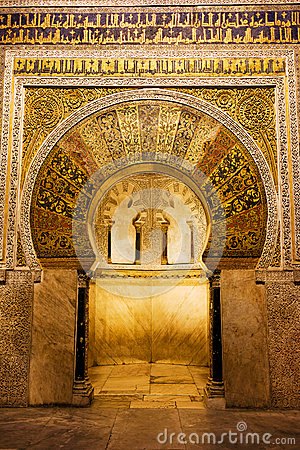
\includegraphics[width=1.40972in,height=2.11458in]{Images/image059.jpg}}{Mihrab dans la mosquée grande de Cordoue}}\label{mihrab-dans-la-mosquuxe9e-grande-de-cordoue}}

\vide{section-29}{%
\subsubsection{{ }{ }}\label{section-29}}

\vide{mihrab-de-cordoue}{%
\mn{{ Mihrab de
Cordoue}{ Mihrab de Cordoue}}\label{mihrab-de-cordoue}}

Il doit précéder sa prière en accomplissant ses ablutions. Elles ont
gagné une certaine importance dans le rite, comme en témoigne le
\emph{ḥadīṯ}~: «~l'ablution est la moitié de la foi~»\sn{~\emph{Ḥadīṯ
  ṣaḥiḥ} rapporté par Muslim ( n°223), Al-Tirmiḏī (n°3517), An-Nasa'ī (
  5/5-6), Ibn Māǧa ( 280 )\label{theol:IbnMaga1}, Ibn Hanbal dans \emph{al-Musnad}.}. Pour cela, il utilise de l'eau, ou à défaut
du sable.

Enfin, il doit formuler l'intention (\emph{niyya}) de faire la prière.
Elle témoigne de la pleine conscience de ce qu'il accomplit.

Que dit al-Ġazālī \label{theol:AlGazali11} de la pratique de la purification~?

Il distingue quatre sens dans ce rituel (Livre 3 de l'\emph{Ihyā'}) :

\begin{itemize}
\item
  la purification extérieure de toute forme de déchets ou de souillures
  diverses. Il s'agit de se purifier des déchets du corps.
\item
  la purification des péchés et des fautes accomplies par le corps
\item
  la purification du cœur de ses vices et de ses mauvais penchants
\item
  la purification du secret intime de tout ce qui n'est pas Dieu.
\end{itemize}

Al-Ġazālī \label{theol:AlGazali12} souligne l'importance de la purification du cœur, de la
purification de toute trace d'idolâtrie à l'époque du Prophète. Or, il
parle de l'obsession de la purification extérieure qui a saisi ses
contemporains et qui est paradoxalement bien loin de celle des Anciens
qui était beaucoup plus profonde. Il parle à cet égard de «~l'idiotie de
la propreté~».

La prière est difficile et la \emph{niyya} ne suffit pas toujours à
garder une concentration fermement tournée vers Dieu. Al-Ġazālī \label{theol:AlGazali13} évoque
les pensées qui sont comme des mouches. De même, la grande mystique de
l'islam Rābi`a disait~: «~Mon Dieu, quand je fais la \emph{ṣalāt},
éloigne de mon cœur toutes les suggestions sataniques (\emph{wasāwis
al-šaytān}), ou alors, par un effet de Ta bonté (\emph{mann}) et de ta
générosité (\emph{karam}), accepte mes prières même troublées par ces
suggestions~»\sn{ʿAttār, \emph{Taḏkīrat al-Awliyā}, cité par
  Badawī p. 157, dans Jean Annestay, p. 101.}.

En islam, \emph{waswas} signifie susurrer à l'oreille, suggérer. Cela
renvoie parfois à une obsession.

\vide{comment-faire-la-priuxe8re}{%
\subsection{{Comment faire la prière~?
}}\label{comment-faire-la-priuxe8re}}

Chaque prière est constitué de la répétition d'un cycle appelé
\emph{rakat}.

Si c'est la première rakat, il s'agit de prononcer la formule
\emph{Allāhu akbar} (\emph{takbīr,} c'est-à-dire c'est le fait de
prononcer cette prière), c'est-à-dire Dieu est plus grand (que tout).
Les mains sont levées au niveau des oreilles et les doigts sont joins.

\vide{httpsupload.wikimedia.orgwikipediacommons44ftakbir_of_prayer.jpg}{%
\mn[
]{\vide{\protect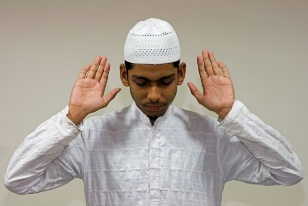
\includegraphics[width=1.38741in,height=0.92708in]{Images/image060.jpg}
}{https://upload.wikimedia.org/wikipedia/commons/4/4f/Takbir\_of\_prayer.jpg }}\label{httpsupload.wikimedia.orgwikipediacommons44ftakbir_of_prayer.jpg}}

Puis il pose la main droite sur sa main gauche au niveau du nombril et
il récite une invocation.

Il demande protection à Dieu avant de réciter la sourate
\emph{al-Fātiha}. Vous vous souvenez, c'est la première sourate du
Coran.

Ensuite, il se prosterne, et en s'abaissant il dit \emph{Allahū akbar.}
Cette position se nomme \emph{ruku}. Il invoque Dieu, puis se redresse,
lève les mains vers les oreilles, puis les rabaisse. Puis il se
prosterne. Cette position se nomme \emph{suǧud}.

\vide{sujud}{%
\mn{{\emph{sujud}}{sujud}}\label{sujud}}

Puis, il s'assoit sur ses genoux et invoque le pardon de Dieu. Il se
prosterne de nouveau et se redresse.

L'ensemble de ce rite s'appelle une \emph{raka}. Il faudra en faire une
ou deux autres.

Pour conclure la prière, le priant salut l'ange de droite et de gauche,
ces anges qui comptabilisent ces bonnes et mauvaises actions pour le
jour du jugement.

Il existe des différences selon les écoles juridiques. Par exemple, le
fait de voir les musulmans se toucher les pieds dans la mosquée est une
prescription du wahhabisme qui date du 18\textsuperscript{ème} siècle~!
Or, elle se généralise, ce qui atteste d'une wahhabisation de l'islam.

Ci-dessous une vidéo récapitulant les gestes, les positions, les paroles
prononcées.

Dans cette explication, beaucoup de choses à remarquer\ldots{} notamment
sur la diversité du rite selon les écoles juridiques (\emph{maḏhab}).

Il est question aussi à plusieurs reprises d'un ouvrage~: \emph{La
citadelle du musulman} qui est un recueil d'invocations selon les
situations de la vie.

À certains moments de la journée, il \textbf{est interdit de faire sa
prière}. Il y aurait là une pédagogie divine. En effet, al-Ġazālī \label{theol:AlGazali14} note
que ce qui est interdit est bien souvent un excitant. De même, les
gestes des différentes postures sont pédagogiques et visent à atténuer
le risque d'ennui. C'est parce que l'on accomplit la prière selon ce
rituel que se polie le cœur.

\emph{Un Récit autour de la prière}

Exemple de Hātim Asamm (le sourd), m. 237/85 \sn{~pour l'anecdote, on l'appelle ainsi,
parce qu'un jour où une vieille femme était venue le consulter, elle
laissa échapper une éructation (expulsion d'un gaz du tube digestif par
la bouche). Pour ne pas embarrasser la femme, il lui demanda de parler
plus fort car il n'entendait pas. La femme fut rassurée, mais pour ce
motif, il joua au sourd 18 années durant, jusqu'à la mort de cette
femme.
}

Donc, «~On lui demandait comment il faisait la prière. Il dit~:
«~D'abord, je purifie mon corps en le lavant avec de l'eau, en même
temps que je lave mon cœur avec la pénitence en faisant une purification
interne. Ensuite, je me rends à la mosquée. En elle je vois la Kaaba, de
même que dans la niche de prière (\emph{mihrāb}) je vois le lieu où se
tenait Abraham. Je distingue à ma droite le Paradis, à ma gauche
l'Enfer, le pont du Sirāt sous mes pieds, Azrā'īl l'ange de la mort
derrière moi. Alors je remets mon cœur à la garde de Dieu, et prononçant
la formule d'entrée en prière `Dieu est grand' (\emph{takbīr}), je joins
mes mains pour la prière, que je fais debout, dans une attitude
suppliante~; je récite le Coran avec soin, je me prosterne en toute
humilité, je reste assis avec persévérance en état d'oraison, et je
finis par l'action de grâce et la salutation~»\sn{\emph{Le
  mémorial des saints}, p. 228-233.}.

\vide{la-zakux101t-limpuxf4t-religieux-purificateur}{%
\section{La zakāt, l'impôt religieux
purificateur}\label{la-zakux101t-limpuxf4t-religieux-purificateur}}



\vide{uxe9tymologie-2}{%
\subsection{Étymologie}\label{uxe9tymologie-2}}

C'est un impôt légal, obligatoire à distinguer de l'aumône libre
\emph{ṣadaqa}.

Étymologiquement, il signifie purifier, croître, prélever.

Cet impôt est lié à la prière~: 
\begin{quote}
    
«~Acquittez-vous de la prière, faites
l'aumône~» (S. 2, 43).
\end{quote}
\vide{bienfaits-de-la-zakux101t}{%
\subsection{{ Bienfaits de la
\emph{zakāt}}}\label{bienfaits-de-la-zakux101t}}

Son but est la circulation des biens et sa répartition équitable. Il
s'agit de faire circuler ce qui est excédent ou superflu~:

\begin{quote}
«~Ils t'interrogent au sujet de ce qu'ils doivent distribuer~? Réponds~:
le superflu~» (S. 2, 219).
\end{quote}

La \emph{zakāt} répond à la nécessité d'enlever l'excédent improductif.
C'est une sorte d'impôt sur la fortune. La \emph{zakāt} doit purifier le
croyant lui-même~: tout est à Dieu. Il doit être responsable devant la
communauté de ce qu'il détient. Ses modalités sont assez complexes et
varient selon les jurisprudences. Initialement, elle ne portait que sur
l'or et l'argent, le bétail, les céréales. Il faut signaler que l'islam
interdit que la monnaie engendre la monnaie et condamne le taux à
intérêt.

Spirituellement, la \emph{zakāt} vise à éprouver le croyant qui prétend
aimer Dieu. Si tu aimes Dieu, alors donne ton superflu. Elle prévient
aussi du danger de prendre l'argent pour Dieu~: elle permet de purifier
le \emph{tawhīd}. C'est-à-dire l'Unicité. Cependant, la \emph{zakāt} ne
doit pas être l'occasion de s'enorgueillir. Il ne faut pas s'en
acquitter publiquement, ce qui constitue aussi une humiliation pour le
pauvre. Le véritable bienfaiteur, ce n'est pas celui qui donne, mais
celui qui reçoit, car il permet à celui qui donne de s'acquitter de ce
qu'il doit donner pour purifier son cœur.

Il s'agit de donner ce qui est licite et ce qui est le plus cher à ses
yeux~: «~Ne choisissez pas ce qui est vil pour donner en \emph{zakāt} »
(S. 2, 267).

\vide{uxe0-qui-donner-la-zakux101t}{%
\subsection{{À qui donner la \emph{zakāt} ?
}}\label{uxe0-qui-donner-la-zakux101t}}

Pour al-Ġazālī \label{theol:AlGazali15}, il faut s'assurer que la personne appartienne à l'une de
ces catégories~:

\begin{itemize}
\item
  elle a la crainte révérencielle~: donc aux pieux, afin de les aider
  dans leur vie spirituelle.
\item
  elle a la science~: donner aux savants, cela contribue à la
  propagation de la foi et de la Loi.
\item
  elle a le sens de la cause première~: autrement dit, elle voit dans le
  don, la manifestation de Dieu. Elle ne s'arrête pas aux moyens, aux
  causes secondes, à la main humaine qui a donné. Cela ne veut pas dire
  qu'elle ne remercie pas le donateur. C'est même une obligation~: celui
  qui n'a pas remercié le donateur n'a pas remercié Dieu.
\item
  elle doit cacher sa pauvreté, ne pas se plaindre.
\item
  elle doit avoir une famille, ou être atteint d'une maladie, croupir
  sous les dettes. La \emph{zakāt} doit lui permettre de sortir de la
  gêne.
\item
  elle doit faire partie des proches et de ceux qui sont liés par le
  sang.
\end{itemize}

\vide{ux1e63iyux101m-et-ux1e63awm-le-jeuxfbne}{%
\section{ṣiyām et ṣawm~: le
jeûne}\label{ux1e63iyux101m-et-ux1e63awm-le-jeuxfbne}}


\vide{ramaux1e0dux101n-mubux101rak}{%
\subsubsection{{\emph{Ramaḍān
mubārak}}{Ramaḍān mubārak}}\label{ramaux1e0dux101n-mubux101rak}}

\vide{duxe9finitions-et-uxe9tymologie}{%
\subsection{Définitions et
étymologie}\label{duxe9finitions-et-uxe9tymologie}}

L'étymologie est intéressante. ṢaWaMa signifie s'abstenir, renoncer à,
s'interdire, se taire, se radoucir en parlant du vent, atteindre le
zénith. Le jeûne a été prescrit au mois de Ramaḍan. Or, RaMaDa renvoie à
l'idée de rôtir, de brûler, d'embraser, d'être brûlant.

\begin{Def}[jeûne]
Le jeûne est donc l'abstention, le silence, l'adoucissement pour
tempérer et neutraliser le feu du mois de Ramadan.
\end{Def}

\mn{Le grand moment liturgique~: c'est le ramadan. On relit le Coran.}
Mais le mois de Ramadan n'est pas qu'affaire de jeûne. Au cours de ce
mois, le musulman est invité à suivre des retraites spirituelles,
notamment les dix derniers jours. Une tradition rapporte~:
\begin{quote}
    «~Dès que
commencent les dix dernières nuits de Ramadan, l'Envoyé de Dieu se
serrait la ceinture, veillait la nuit en dévotion et réveillait les gens
de sa maison~»
\end{quote}. Selon les savants, l'expression «~se serrer la
ceinture~» signifie se détourner des femmes pour montrer tout le sérieux
dans son action spirituelle.

Le but du jeûne est donc spirituel~: parce que l'homme est une créature
entre l'animal et l'ange, s'il se soumet à ses passions, il et ramené à
l'état bestial, mais s'il les combat, il s'élève à celui des anges car
supporter la faim et la soif est un attribut de Dieu et des anges.

\vide{diffuxe9rents-types-de-jeuxfbne}{%
\subsection{4.2 Différents types de
jeûne}\label{diffuxe9rents-types-de-jeuxfbne}}

\emph{Ṣiyām} qualifie le jeûne obligatoire~; c'est le jeûne légal de
prescription divine. Il est un exercice de soumission volontaire, le
bouclier de la chasteté quand on ne peut pas se marier~; le jeûne
consiste aussi en l'abstention de tout mal, en paroles et en actes.

Al-Ġazālī \label{theol:AlGazali16} distingue trois sortes de jeûnes~:

\begin{itemize}
\item
  Le jeûne des gens du commun~: on s'abstient de manger ou de boire,
  d'avoir des rapports sexuels.
\item
  le jeûne des gens de l'élite~: empêcher le regard, la langue, la main,
  le pied, l'ouïe, la vue et l'ensemble des membres de commettre des
  péchés.
\item
  le jeûne de l'élite de l'élite~: c'est le jeûne du cœur devant les
  basses ambitions et les idées qui éloignent de Dieu.
\end{itemize}

Le jeûne n'est pas purement abstinence~: il est associé à la nécessité
de la réconciliation, de la générosité, de l'hospitalité. On peut citer
à cet égard le \emph{ḥadīṯ}~suivant : \emph{«~Pour celui qui ne renonce
pas au mensonge dans les actes et les paroles, Dieu n'a nul besoin qu'il
renonce à sa nourriture et à sa boisson}~».

\emph{ṣawm} qualifie le jeûne libre. Le jeûne n'est pas spécifique au
mois du Ramadan. Les musulmans sont invités à jeûner au début et à la
fin de chaque mois, ou trois jours au milieu. On doit aussi jeûner le
jour de \emph{ʿarafāt} ou de \emph{ʿāšūrāʾ}. Vous ne connaissez pas ces
deux mots. Pas de panique. Cela viendra et je vous enverrai un petit
pensum\ldots{}

Le jeûne a une dimension spirituelle. Il est abstention et attitude
intérieure. Il va faire ressortir dans l'être un certain nombre
d'appétits, de dispositions, de traits de caractère qui ne sont pas
conformes à une orientation tournée vers Dieu seul. Il va révéler les
tendances troubles qui sont en nous, les tendances troubles de l'âme qui
sommeillent et nous trompent. Le jeûne va donc purifier l'être, le
rendre transparent comme un diamant afin de rendre présent Dieu seul.

Si vous lisez le livre qu'al-Ġazālī \label{theol:AlGazali16} consacre au jeûne, vous verrez qu'il
critique la tendance de certains de sa communauté à s'abstenir
d'aliments et de boissons dans la journée mais à s'empiffrer dès que le
soleil est tombé. Il y a pour le savant une profonde méprise et
perversion du rite.

\vide{le-puxe8lerinage-le-ux1e25aux11fux11f}{%
\section{{Le pèlerinage~: le \emph{ḥağğ}
}}\label{le-puxe8lerinage-le-ux1e25aux11fux11f}}


\vide{uxe9tymologie-3}{%
\subsection{{ Étymologie
}}\label{uxe9tymologie-3}}

La racine Ḥa Ğa Ğa signifie se diriger vers, se proposer, l'emporter
dans l'argumentation sur quelqu'un.

Le \emph{ḥağğ} est donc une quête. Il regroupe l'ensemble des actes
accomplis au cours du Pèlerinage. Il correspond au Pèlerinage que
Muḥammad a accompli en l'an dix de l'Hégire, quelques mois avant sa
mort, avec 140~000 musulmans. C'est le Pèlerinage de l'Adieu,
\emph{ḥiğğat al-Wadā`.} Le neuvième jour du douzième mois, fut révélé à
Muḥammad le verset suivant~: «~Ce jour, j'ai parachevé pour vous votre
religion. J'ai parachevé mon Bienfait à votre égard et j'agrée pour vous
l'islam comme religion~» (S. 5, 3).

La révélation a lieu à Arafat, situé en dehors du territoire sacré.

Le \emph{ḥaǧǧ} est une obligation pour tout musulman qui en a les
moyens.

On distingue le petit \emph{ḥağğ} du grand \emph{ḥağğ}~: le premier est
fait n'importe quand dans l'année tandis que le second est effectué
seulement pendant le mois du Ramaḍān.

\vide{conditions-requises-uxe0-laccomplissement-du-ux1e25aux11fux11f}{%
\subsection{{Conditions requises à l'accomplissement
du \emph{ḥağğ}
}}\label{conditions-requises-uxe0-laccomplissement-du-ux1e25aux11fux11f}}

\begin{itemize}
\item
  Des dépenses d'origine licite
\item
  Ne pas aider les ennemis de Dieu en leur versant des droits d'entrée
\item
  Des dépenses faites avec parcimonie
\item
  La chasteté est de rigueur dans les propos~: on doit s'encourager, se
  stimuler spirituellement.
\item
  Se préparer au grand voyage, comme si on n'allait pas revenir.
\end{itemize}

\vide{le-rituel}{%
\subsection{Le rituel}\label{le-rituel}}

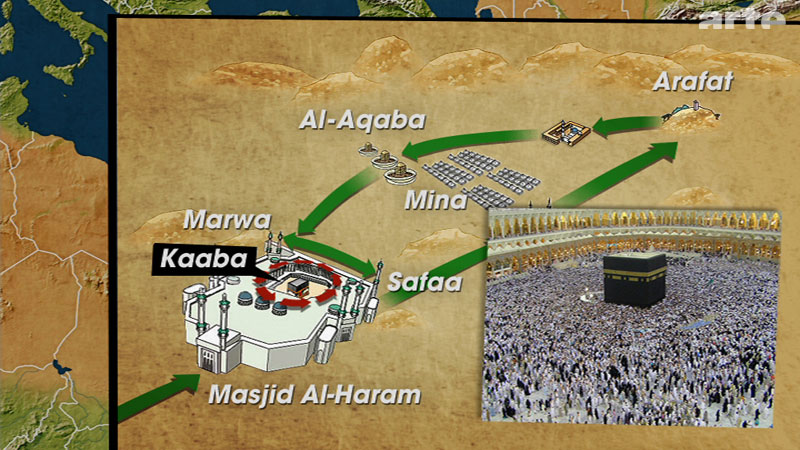
\includegraphics[width=5.51181in,height=3.09931in]{Images/image066.jpg}

Tout commence à la limite du territoire sacré. On exprime la
\emph{niyya}. Le mot a été rencontré à propos de la prière. Quand on
commence à faire la prière, il faut formuler la \emph{niyya}
c'est-à-dire\ldots~? Allez, un petit effort, je suis sûr que vous le
savez.

Puis, il s'ensuit un rituel vestimentaire et corporel qui donne le
statut d'\emph{iḥrām}, c'est-à-dire de consécration. On procède à la
grande ablution. Puis on revêt un vêtement composé de deux pièces
d'étoffes blanches non cousues.

On ne doit pas se couper les cheveux, s'épiler, se couper les ongles, se
couvrir la tête pour l'homme, chasser ou avoir des relations sexuelles.

Le pèlerin va vers la Kaaba, temple selon la tradition musulmane
construit par Adam, reconstruit par Abraham. On y trouve la pierre noire
(blanche à l'origine, mais devenue noire à cause des péchés des hommes.
Sur cette pierre, il existe plusieurs légendes).

Le pèlerin marche autour du Temple. Sa déambulation se dénomme
\emph{tawaf}. À l'approche de la Mosquée, il lève les deux bras vers le
Ciel et répète~: \emph{Labbayka Allahouma Labbayka} (Me voici, ô mon
Dieu, me voici).

Dans la mosquée, il doit toucher la pierre noire, ou faire un geste en
sa direction.

Le fidèle fait 7 fois le tour de la Kaaba, trois rapides et 4 lents dans
le sens inverse des aiguilles d'une montre. C'est la giration autour du
centre de l'univers.

Puis vient le \emph{say}, ou course angoissée d'Agar. Agar est cette
femme, servante de Sarah, qui fut chassée par sa maîtresse. Elle dut
fuir dans le désert, avec dans ses bras son enfant, Ismaël. Elle cherche
de l'eau, puis surgit la source de Zemzem. Le pèlerin accomplit cette
marche entre deux rochers distants de 400m, Safa et Marwa. Il doit faire
la course 7 fois. À la fin, il boit de l'eau de Zemzem.

Ces rites accomplis, on entre dans le cœur du pèlerinage. C'est le 8 de
\emph{Dhou al-hijja}, le dernier mois de l'année lunaire. Le pèlerin se
rend à pied à Mina, à 7 km de La Mecque et il y campe. Il reçoit le
pardon de Dieu (\emph{woukouf}). Il marche vers la plaine d'Arafat à 12
km. À midi, station debout prolongée où le pèlerin reçoit le pardon de
Dieu au pied du mont de la Miséricorde (\emph{Ğabal al-Raḥma})~: c'est
de là que Muḥammad s'adressa aux fidèles lors de son pèlerinage d'Adieu.
C'est le point culminant du pèlerinage. Puis on revient sur ses pas, le
soir, on s'arrête à Mouzdalifa pour y passer la nuit. Là, on ramasse les
49 petits cailloux pour les lapidations rituelles des stèles
représentant le démon.

C'est l'\emph{Aïd al-Ada} ou la fête du sacrifice d'Abraham.

Le 10 du mois, avant l'Aube, on se rend à Mina pour une lapidation
symbolique et pour y sacrifier un animal. C'est l'\emph{Aïd al-Kebir}.
Après le sacrifice, le pèlerin se coupe les cheveux ou se les rase.

Le \emph{Tawaf} est la marche d'Adieu autour du Temple. Le 11 et le 12
ont lieu d'autres lapidations symboliques. Les fidèles reviennent à La
Mecque pour la circumambulation de l'Adieu autour de la Kaaba. Le
pèlerinage est fini. Certains le complètent par un voyage à Médine.

\vide{conclusion-1}{%
\section{Conclusion~}\label{conclusion-1}}

Pour conclure, une histoire, celle d'un dialogue entre Moïse et Dieu et
qui tend à minimiser l'importance de ces 5 piliers pour privilégier la
voie de l'amour mais aussi celle de l'aversion.

\begin{quote}
«~On rapporte que Dieu a révélé à Moïse~: «~As-tu jamais accompli une
œuvre pour Moi~? Moïse répondit~: Mon Dieu~! J'ai prié devant Toi~; j'ai
jeûné, j'ai fait l'aumône légale~! Dieu lui dit~: la prière est pour toi
une preuve (burhān), le jeûne une armure (ğunna), l'aumône est un abri
(ẓill), l'impôt légal une lumière (nūr). Mais quelle œuvre as-tu fait
pour Moi~? Moïse dit~: Mon Dieu~! Indique-moi quelle est l'œuvre qui
soit à Toi~? Dieu lui dit~: Ô Moïse, as-tu jamais pris un ami pour moi~
et en animosité un ennemi pour Moi~? Moïse sut alors que la meilleure
œuvre c'est l'amour en Dieu et l'aversion en Dieu~»\sn{Al-Ġazālī \label{theol:AlGazali9}\emph{,
  Les règles de l'amitié et de la fraternité en Islam}, (K. 15, ar. p.
  593~; fr. p. 19) {[}notre traduction{]}.}.
\end{quote}

\textbf{Pour aller plus loin~:}

On pourra lire le récit passionnant d'Abdallah Hammoudi, anthropologue
et enseignant à Princeton~: \emph{Une saison à La Mecque}, Paris, Seuil,
2005. Il s'agit à la fois d'une démarche de croyant et d'anthropologue.
Mais les deux sont-ils compatibles~? À son retour au Maroc, Hammoudi
refusera le titre de \emph{hāǧ} que l'on attribue à celui qui revient de
pèlerinage. Un signe manifeste de la difficulté qu'il a rencontrée à
concilier la démarche scientifique, objective, observatrice, et sa
participation comme musulman.

\vide{httpwww.seuil.comimagescouvm9782020669801.jpg}{%
{{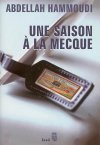
\includegraphics[width=1.04167in,height=1.51389in]{Images/image067.jpg}}{http://www.seuil.com/images/couv/m/9782020669801.jpg}}\label{httpwww.seuil.comimagescouvm9782020669801.jpg}}
